% Editable simulator report. Figures are compiled separately from Typst.
% Build from this directory with uv run python simulator_report/scripts/build_latex.py.
\RequirePackage{fix-cm}
\documentclass[10pt,letterpaper]{article}
\usepackage[margin=0.72in,headheight=15pt]{geometry}
\usepackage[T1]{fontenc}
\usepackage[utf8]{inputenc}
\usepackage{times,amsmath,amssymb,textcomp}
\renewcommand{\ttdefault}{cmtt}
\usepackage{graphicx,float,booktabs,longtable,array,calc}
\usepackage{enumitem,titlesec,fancyhdr,xcolor}
\usepackage[numbers,sort&compress]{natbib}
\usepackage{xurl}
\usepackage[hidelinks]{hyperref}
\usepackage{verbatim}
\makeatletter
\def\verbatim@font{\normalfont\ttfamily\footnotesize}
\makeatother
\definecolor{navy}{HTML}{17324D}
\definecolor{teal}{HTML}{0B6E75}
\definecolor{pale}{HTML}{EAF3F3}
\definecolor{slate}{HTML}{5B6573}
\setlength{\parindent}{0pt}
\setlength{\parskip}{6pt}
\setlength{\emergencystretch}{2em}
\setlist[itemize]{leftmargin=1.4em,itemsep=2pt,parsep=1pt,topsep=4pt}
\setlist[itemize,1]{label=\textbullet}
\setlist[itemize,2]{label=--}
\setlist[itemize,3]{label=\rule{0.35em}{0.35em}}
\titleformat{\section}{\color{navy}\bfseries\fontsize{17}{19}\selectfont}{\thesection}{0.6em}{}
\titleformat{\subsection}{\color{navy}\bfseries\fontsize{12}{14}\selectfont}{\thesubsection}{0.6em}{}
\titleformat{\subsubsection}{\color{navy}\bfseries}{\thesubsubsection}{0.6em}{}
\titlespacing*{\section}{0pt}{14pt}{7pt}
\titlespacing*{\subsection}{0pt}{10pt}{5pt}
\newenvironment{reportnote}{\begin{quote}\small\color{navy}}{\end{quote}}
\pagestyle{fancy}
\fancyhf{}
\fancyhead[L]{\small\color{slate}BLUEBOAT SIMULATOR}
\fancyhead[R]{\small\color{slate}J.C. Vaught}
\fancyfoot[C]{\thepage}
\renewcommand{\headrulewidth}{0pt}
\hypersetup{pdftitle={BlueBoat Configurable Simulator. Design and Verification},pdfauthor={J.C. Vaught}}
\begin{document}
\fontsize{10.5}{12.6}\selectfont
{\color{navy}\fontsize{25}{28}\selectfont BlueBoat Configurable Simulator\par}
\vspace{4pt}
{\fontsize{16}{18}\selectfont Design, assumptions, configuration, and verification\par}
\vspace{8pt}
J.C. Vaught\hfill October 13, 2026
\vspace{10pt}

The simulator supplies a repeatable environment for developing boat controllers. It separates hull motion, M200 propulsion, command execution, and sensor delivery so that each assumption can be tested independently. This report documents the implemented equations and information flow, gives the complete flag reference, and explains the saved model comparisons.

\begin{itemize}
\item
  Begin with a local linear plant around a declared operating speed.

  \begin{itemize}
  \item
    Add nonlinear hull and propulsion effects, then motor response, timing, sensing, and disturbances.

    \begin{itemize}
    \item
      Compare identical commands and initial conditions before attributing a change to the selected feature.
    \end{itemize}
  \end{itemize}
\item
  Keep simulated motion separate from controller observations.

  \begin{itemize}
  \item
    The internal state supplies numerical integration and scoring; measurement delivery supplies the future feedback interface.

    \begin{itemize}
    \item
      An explicit perfect-state switch supports ideal controller tests. Ordinary sensor tests require an estimator.
    \end{itemize}
  \end{itemize}
\item
  Distinguish implementation verification from boat validation.

  \begin{itemize}
  \item
    Automated checks establish consistency, causality, bounds, and repeatability.

    \begin{itemize}
    \item
      Measured boat logs establish predictive accuracy. Added model detail does not by itself establish improvement.
    \end{itemize}
  \end{itemize}
\end{itemize}

\begin{reportnote}

The saved demonstration uses an open-loop command program. The companion controller report adds proportional-integral-derivative control, linear quadratic regulation, pole placement, and state estimation through the same motor-percentage interface.

\end{reportnote}

The physical demonstration follows baseline revision \texttt{ea307b3}, with its commands now expressed as signed motor percentages. The companion controller report supplies the subsequently implemented feedback study. Its diagrams use a dedicated navy-and-teal language, and its quantitative charts use standard plot colors. Every figure is authored in Typst with CeTZ or Lilaq, with inspectable source data retained beside the chapters.

\clearpage\tableofcontents\clearpage

\section{Hull dynamics}

The simulator advances a planar hull state from body-frame velocities and two independently commanded propulsors. This chapter defines its coordinate convention, derives the implemented equations, and relates the linear baseline to the nonlinear hull model.

\subsection{Frames and state}

The inertial frame uses east \(E\) and north \(N\) position coordinates. The body frame uses forward \(x_{b}\) and port/left \(y_{b}\) axes, with heading \(\psi\) measured counterclockwise from east. Consequently, a zero-heading boat points east, while a positive heading rotates its forward axis toward north. Surge \(u\), sway \(v\), and yaw rate \(r\) are body-frame velocities. The six-state hull vector is \(\eta = (E,N,\psi)\) and \(\nu = (u,v,r)\).


\begin{figure}[H]
\centering
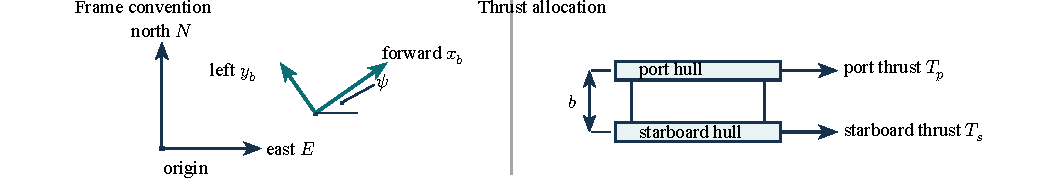
\includegraphics[width=\linewidth]{simulator_report/figures/standalone/01_coordinates.pdf}
\caption{Body forward and left axes rotate with heading, while east and north remain fixed.}
\label{fig:dyn-coordinates}
\end{figure}


That convention fixes both the position rotation and the sign of differential thrust. The exact kinematic relation is

\begin{equation}
\dot{E} = \cos(\psi)u - \sin(\psi)v,\quad\dot{N} = \sin(\psi)u + \cos(\psi)v,\quad\dot{\psi} = r.
\end{equation}

In matrix form, \(\dot{\eta} = J(\psi)\nu\), where the planar rotation block is

\begin{equation}
J(\psi) = \begin{pmatrix}
\cos(\psi) & - \sin(\psi) & 0 \\
\sin(\psi) & \cos(\psi) & 0 \\
0 & 0 & 1
\end{pmatrix}.
\end{equation}

The two frames keep position and velocity descriptions consistent as the craft turns.

\begin{itemize}
\item
  The earth frame records where the hull is, while the body frame records how it moves relative to its own axes.

  \begin{itemize}
  \item
    Surge is forward and sway is left, so the body axes rotate together with heading.
  \item
    Applying \(J(\psi)\) resolves these velocities into east and north components at every step.
  \end{itemize}
\item
  Heading is positive counterclockwise from east.

  \begin{itemize}
  \item
    At \(\psi = 0\), forward points east; at positive \(\psi\), forward has a northward component.
  \item
    This sign convention makes positive yaw and a larger starboard thrust produce a counterclockwise turn.
  \end{itemize}
\end{itemize}

\subsection{Nonlinear planar force balance}

The force model follows the standard marine-craft decomposition of inertia, velocity coupling, damping, and applied effort. Here each term is specified by the implementation and configuration; the general modeling framework is consistent with Fossen's marine craft formulation \cite{Fossen2026MarineModel}.

The effective diagonal inertia is \(M = \operatorname{diag}\left( m_{x},m_{y},I_{z} \right)\). The nominal rigid-body yaw inertia is \(I\), while \(I_{z}\) denotes its effective value after the optional added-inertia contribution. With rigid-body mass \(m\) and added-mass flag \(a \in \left\{ 0,1 \right\}\), code sets

\begin{equation}
m_{x} = m(1 + 0.10a),\quad m_{y} = m(1 + 0.50a),\quad I_{z} = I(1 + 0.20a).
\end{equation}

The implemented velocity-coupling vector added on the right-hand side is \(c(\nu) = \left( m_{y}vr, - m_{x}ur,\left( m_{x} - m_{y} \right)uv \right)^{T}\). Under the conventional left-hand-side form \(M\dot{\nu} + C(\nu)\nu = \tau\), this is \(c(\nu) = - C(\nu)\nu\). Its structure exchanges energy between surge, sway, and yaw without adding or removing total kinetic energy, since

\begin{equation}
\nu^{T}c(\nu) = um_{y}vr - vm_{x}ur + r\left( m_{x} - m_{y} \right)uv = 0.
\end{equation}

This cancellation is a useful structural check on the cross-coupling signs. The model's body-frame equations are

\begin{equation}
m_{x}\dot{u} = T_{p} + T_{s} + m_{y}vr - D_{u}(u) + \tau_{u}.
\end{equation}

\begin{equation}
m_{y}\dot{v} = - m_{x}ur - D_{v}(v) + \tau_{v}.
\end{equation}

\begin{equation}
I_{z}\dot{r} = \frac{b}{2}\left( T_{s} - T_{p} \right) + \left( m_{x} - m_{y} \right)uv - D_{r}(r) + \tau_{r}.
\end{equation}

Here \(T_{p}\) and \(T_{s}\) are port and starboard thrust in newtons, \(b\) is their lateral separation, and \(\left( \tau_{u},\tau_{v},\tau_{r} \right)\) denotes environmental surge force, sway force, and yaw moment in body coordinates. Positive differential effort means starboard thrust exceeds port thrust and therefore produces positive, counterclockwise yaw.

The drag laws are signed so that they oppose velocity. In nonlinear mode they are

\begin{equation}
D_{u}(u) = d_{1}u + d_{2}u|u|,\quad D_{v}(v) = d_{v}v + k_{v}v|v|,\quad D_{r}(r) = d_{r}r + k_{r}r|r|.
\end{equation}

Configuration defaults set \(k_{v} = k_{r} = 0\). Thus default lateral and yaw drag are linear, while surge drag combines linear and quadratic terms. The quadratic surge term captures increasing resistance with speed while retaining the correct sign in reverse.


\begin{figure}[H]
\centering
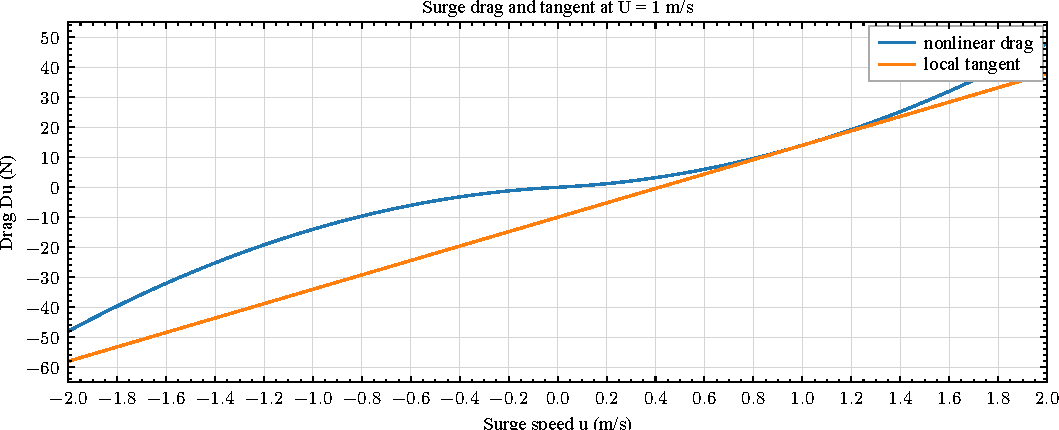
\includegraphics[width=\linewidth]{simulator_report/figures/standalone/02_surge_drag.pdf}
\caption{The straight-line approximation matches nonlinear surge drag and slope at the one-meter-per-second operating point.}
\label{fig:dyn-drag}
\end{figure}


\subsection{Hull and coefficient values}

The numeric hull begins with the 1.2 m length and 0.93 m beam of the configured platform. The implementation computes a 21.9 kg rigid-body mass as 14.5 kg bare hull plus 2.4 kg for two batteries and a 5.0 kg equipment allowance. The nominal yaw inertia uses a uniform rectangular-envelope approximation, \(I = \frac{m\left( L^{2} + B^{2} \right)}{12} = 4.2064425\) kg m\textsuperscript{2}. This is a geometry-based modeling choice, not a measured mass distribution. Thruster spacing is configured as \(b = 0.75\) m.

The configured values combine platform dimensions, mass accounting, and assumed resistance coefficients.

\begin{itemize}
\item
  Platform geometry and mass determine the rigid-body terms.

  \begin{itemize}
  \item
    The 1.2 m length, 0.93 m beam, 14.5 kg bare hull, and 2.4 kg battery total are platform specifications; the 5.0 kg equipment allowance is a configuration assumption.
  \item
    Together they produce \(m = 21.9\) kg; the 0.75 m thruster separation is also a configuration assumption.
  \end{itemize}
\item
  The inertia proxy converts the platform envelope into yaw resistance.

  \begin{itemize}
  \item
    The model uses \(I = \frac{m\left( L^{2} + B^{2} \right)}{12} = 4.2064425\) kg m\textsuperscript{2}, giving \(I_{z} = I\) when added mass is off.
  \item
    With added mass on, the configured fractions give \(m_{x} = 24.09\) kg, \(m_{y} = 32.85\) kg, and \(I_{z} = 5.047731\) kg m\textsuperscript{2}.
  \end{itemize}
\item
  Drag coefficients set the resistance used by the hull equations.

  \begin{itemize}
  \item
    The assumed surge terms are \(d_{1} = 4\) N s/m and \(d_{2} = 10\) N s\textsuperscript{2}/m\textsuperscript{2}; sway and yaw use \(d_{v} = 35\) N s/m and \(d_{r} = 12\) N m s.
  \item
    The configuration defaults omit quadratic sway and yaw drag, so \(k_{v} = k_{r} = 0\).
  \end{itemize}
\end{itemize}

Thrust allocation maps the two motors to generalized effort as

\begin{equation}
\tau_{T} = \begin{pmatrix}
1 & 1 \\
0 & 0 \\
 - \frac{b}{2} & \frac{b}{2}
\end{pmatrix}\begin{pmatrix}
T_{p} \\
T_{s}
\end{pmatrix}.
\end{equation}

At \(b = 0.75\) m, equal thrust changes surge without yaw, while an equal-and-opposite change creates yaw with no net surge. Installed thrust is based on a signed static motor curve scaled so the pair reaches the platform's stated 8.2 kgf forward maximum. Reverse scaling and between-point values remain assumptions in that map; the hull force equations themselves consume thrust in newtons.

\subsection{Local linear model and feature switches}

The initial configuration holds \(U = 1\) m/s and \(\psi_{0} = 0\). The nominal position evolves as \(E_{0}(t) = Ut\) and \(N_{0}(t) = 0\), so \(\widetilde{E} = E - E_{0}(t)\) and \(\widetilde{N} = N - N_{0}(t)\) describe departures from that moving reference. For small velocity and heading perturbations \(\widetilde{u},\widetilde{v},\widetilde{r},\widetilde{\psi}\), with trim thrust balancing drag, the linearized equations are

\begin{equation}
\dot{\widetilde{E}} = \widetilde{u}.
\end{equation}

\begin{equation}
\dot{\widetilde{N}} = \widetilde{v} + U\widetilde{\psi}.
\end{equation}

\begin{equation}
\dot{\widetilde{\psi}} = \widetilde{r}.
\end{equation}

\begin{equation}
\dot{\widetilde{u}} = - \left( \frac{d_{1} + 2d_{2}U}{m_{x}} \right)\widetilde{u} + \frac{\widetilde{T_{p}} + \widetilde{T_{s}}}{m_{x}}.
\end{equation}

\begin{equation}
\dot{\widetilde{v}} = - \left( \frac{d_{v}}{m_{y}} \right)\widetilde{v} - \left( m_{x}\frac{U}{m_{y}} \right)\widetilde{r}.
\end{equation}

\begin{equation}
\dot{\widetilde{r}} = \left( \left( m_{x} - m_{y} \right)\frac{U}{I_{z}} \right)\widetilde{v} - \left( \frac{d_{r}}{I_{z}} \right)\widetilde{r} + \frac{b\left( \widetilde{T_{s}} - \widetilde{T_{p}} \right)}{2I_{z}}.
\end{equation}

These equations give a readable state-space model \(\dot{\widetilde{x}} = A\widetilde{x} + B\widetilde{T}\) for \(\widetilde{x} = \left( \widetilde{E},\widetilde{N},\widetilde{\psi},\widetilde{u},\widetilde{v},\widetilde{r} \right)\) and \(\widetilde{T} = \left( \widetilde{T_{p}},\widetilde{T_{s}} \right)\). For the default no-added-mass coefficients, the nonzero entries of \(A\) are \(A_{E,u} = 1\), \(A_{N,v} = 1\), \(A_{N,\psi} = U = 1\) m/s, \(A_{\psi,r} = 1\), \(A_{u,u} = - 1.0959\) s\textsuperscript{-1}, and \(A_{v,v} = - 1.5982\) s\textsuperscript{-1}, \(A_{v,r} = - 1.0000\) m/s, \(A_{r,r} = - 2.8523\) s\textsuperscript{-1}. The input matrix rows for \(u\) are \((0.04566,0.04566)\) kg\textsuperscript{-1}; rows for \(r\) are \(( - 0.08915,0.08915)\) with units kg\textsuperscript{-1} m\textsuperscript{-1}. All other entries of \(A\) are zero.

The feature flags select whether this local approximation or the corresponding nonlinear relation supplies each component.

\begin{itemize}
\item
  \texttt{nonlinear\_kinematics} switches from the local position approximation to exact rotation at the current heading. At heading zero it uses lateral velocity \(v + U\left( \psi - \psi_{0} \right)\), retaining the first-order effect of heading on cross-track motion.

  \begin{itemize}
  \item
    Near \(U = 1\) m/s and small heading error, this agrees to first order with exact rotation. Large heading changes require the nonlinear rotation.
  \end{itemize}
\item
  \texttt{nonlinear\_coupling} replaces the constant-speed linear terms \(\left( - m_{x}Ur,\left( m_{x} - m_{y} \right)Uv \right)\) with the full state-dependent terms \(\left( m_{y}vr, - m_{x}ur,\left( m_{x} - m_{y} \right)uv \right)\).

  \begin{itemize}
  \item
    The local coupling evaluates sway/yaw cross terms at trim speed \(U\) and discards nonlinear state products.
  \end{itemize}
\item
  \texttt{nonlinear\_drag} replaces the tangent drag law around \(U\) with signed quadratic surge drag and configured sway/yaw quadratic terms.

  \begin{itemize}
  \item
    In surge, linear mode evaluates \(D_{u}(U) + \left( d_{1} + 2d_{2}|U| \right)(u - U)\). It is accurate near the trim speed and diverges increasingly from the nonlinear curve farther away.
  \end{itemize}
\item
  \texttt{added\_mass} scales the diagonal effective inertia by the configured fractions and changes the coupling coefficients through \(m_{x},m_{y},I_{z}\).
\end{itemize}

Accordingly, the baseline is a local model for small perturbations around its selected speed and heading. Turning on the \texttt{01\_hull} preset restores exact position rotation, nonlinear coupling, and nonlinear drag, while preserving the same mass and nominal coefficient choices. These equations describe the implemented hull dynamics; motor response, command timing, sensors, and disturbances are separate simulator layers.

\section{Actuation and Command Timing}\label{actuation-chapter}

\subsection{From motor percentage to thrust}

The propulsion model starts from Blue Robotics' signed M200 static samples at 16 V, then scales both motors uniformly to match the BlueBoat's published 8.2 kgf forward rating. This joins a component curve to an installed-boat rating as a provisional model assumption. The product information supplies the 8.2 kgf figure, and the retained technical-reference samples supply the M200 curve \cite{BlueRobotics2026M200Reference}\cite{BlueRobotics2026BlueBoatProduct}.

Signed motor command \(a\) runs from -100\% full reverse through 0\% neutral to +100\% full forward. It denotes normalized drive request, rather than percent thrust or power. The adapter converts this to the device pulse width \(p\) before evaluating the retained map.

\begin{equation}
p(a) = (1500 + 4a)\text{ \textmu{}s}.
\end{equation}

The force assigned to a motor follows

\begin{equation}
F_{\text{inst}(p)} = sF_{16}(p),\quad s = \left( 8.2\text{ kgf} \right)\frac{9.80665\frac{\text{ N}}{\text{kgf}}}{2\max\limits_{p}F_{16}(p)}.
\end{equation}

Here \(F_{16}\) is the piecewise-linear interpolation of the retained 16 V samples, and \(s = 0.72824\) is dimensionless. The result sets the positive limit to \(40.207N\) per motor and the native reverse limit to \(- 20.068N\) per motor. The forward limit is anchored to the product rating. Uniform scaling of reverse and intermediate values is the model's installation assumption.


\begin{figure}[H]
\centering
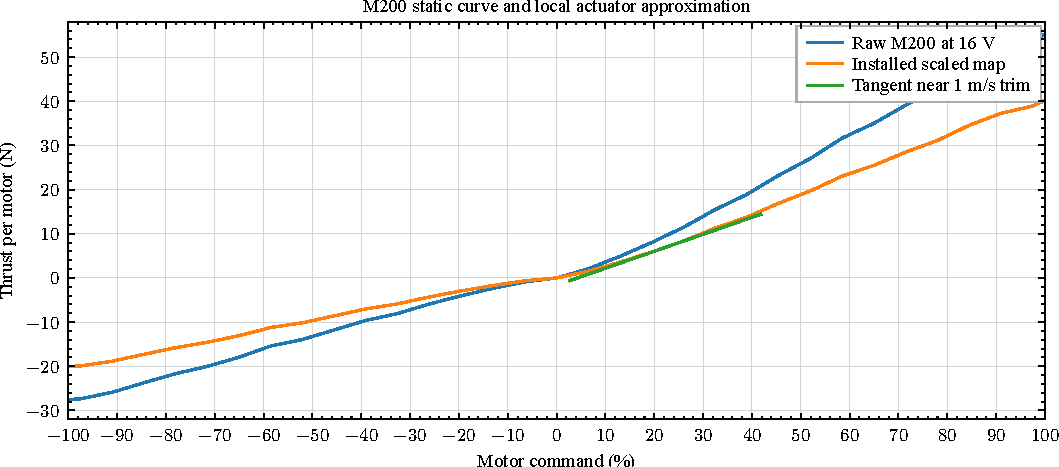
\includegraphics[width=\linewidth]{simulator_report/figures/standalone/03_thrust_map.pdf}
\caption{The installed map matches the pair's forward rating; the tangent is local to trim.}
\label{fig:actuation-thrust-map}
\end{figure}


The simulator offers two actuator descriptions so the experiment can isolate nonlinear effects from a local approximation.

\begin{itemize}
\item
  The nonlinear lookup path uses the installed curve. Input percentages stay within -100\% through +100\%; the saturation flag also bounds force.

  \begin{itemize}
  \item
    With neutral deadband enabled, commands from -6.25\% through +6.25\% produce zero thrust.
  \item
    With reverse asymmetry enabled, commands below neutral use the signed reverse branch, retaining the lower reverse limit. When disabled, the model mirrors the forward branch into reverse and therefore removes the measured map asymmetry.
  \end{itemize}
\item
  The local model computes \(F = F_{0} + k_{a}\left( a - a_{0} \right)\) around a selected trim.

  \begin{itemize}
  \item
    At 1 m/s, the standard linear and quadratic surge drag values require \(7.0N\) per motor. The map gives \(a_{0} = 22.475\) percent, with local slope \(k_{a} = 0.38455\) N per percentage point.
  \item
    At 25\%, both predict \(7.971N\) because trim and 25\% lie in the same piecewise-linear map segment. At 50\%, the lookup gives \(18.854N\) while the tangent extrapolation gives \(17.585N\), a \(1.269N\) difference.
  \end{itemize}
\end{itemize}

The force path also allows a channel mismatch after percentage-to-force conversion. Port and starboard gains default to 0.95 and 1.05, then thrust bounds are reapplied if saturation is active. For example, at the plotted 50\% command, the native installed lookup gives \(18.85N\) before channel gains. The channel targets become \(17.91N\) and \(19.80N\), so equal percentage commands can create a \(1.89N\) thrust difference and an unintended yaw moment.

\subsection{Motor response after a command}

Once an applied command sets a new target, the simulator evolves motor force with an optional first-order lag and optional force slew limit. With lag time constant \(\tau\) and rate limit \(R\), define error magnitude \(m = |F_{t} - F_{0}|\), direction \(q \in \left\{ - 1,0,1 \right\}\) from current force toward target, and transition time \(t_{r} = \frac{\max(m - R\tau,0)}{R}\). The remaining error is

\begin{equation}
e(t) = \begin{cases}
m-Rt, & 0\leq t\leq t_r, \\
\min(m,R\tau)\exp\!\left(-\dfrac{t-t_r}{\tau}\right), & t>t_r.
\end{cases}\quad F(t) = F_{t} - qe(t).
\end{equation}

This combined law initially slews at up to \(R\) and then follows the first-order exponential tail. When only lag is enabled, the full response is exponential. When only the rate limit is enabled, force moves at constant rate until it reaches the target. With both features disabled, target force applies immediately.


\begin{figure}[H]
\centering
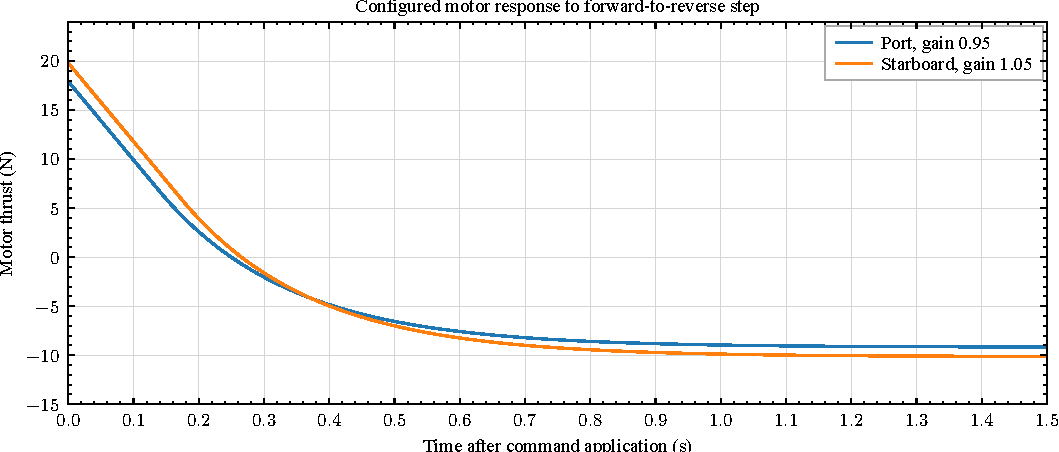
\includegraphics[width=\linewidth]{simulator_report/figures/standalone/04_motor_reversal.pdf}
\caption{Motor force response to a +50\% to -50\% reversal after the target applies.}
\label{fig:actuation-reversal-response}
\end{figure}


For this plotted reversal, each motor changes target from forward to reverse while its state starts at the corresponding 50\% steady force. The port target moves from \(17.91N\) to \(- 9.17N\), and the starboard target moves from \(19.80N\) to \(- 10.14N\). With \(\tau = 0.2s\) and \(R = 80\frac{N}{s}\), the port error magnitude is \(27.09N\) and the linear portion lasts about \(0.139s\), followed by an exponential tail. The starboard linear portion lasts about \(0.174s\). The delay from command decision to applied target is separate from these motor dynamics.

\subsection{Command clock and delivery faults}

When command sampling is enabled, the configured \(20\text{ ms}\) period gives a 50 Hz decision rate. When command delay is enabled, each command then passes through three configured delay terms: \(5\text{ ms}\) for computation, \(10\text{ ms}\) for transport, and \(20\text{ ms}\) of actuator dead time. Their nominal sum is \(35\text{ ms}\), or 1.75 command periods. Optional timing jitter adds a uniform value from zero to \(3\text{ ms}\) per decision. Because delayed commands are queued as events, more than one command may be in flight.

\begin{itemize}
\item
  Sampling and delays affect when a new percentage pair can change the target.

  \begin{itemize}
  \item
    A missed update creates no application event, so the previously applied percentage and force target remain in effect.
  \item
    The default missed-command probability is zero; fault experiments can raise it.
  \end{itemize}
\item
  The optional watchdog monitors applied command freshness.

  \begin{itemize}
  \item
    Its default timeout is \(100\text{ ms}\). Each applied command schedules a timeout, and newer applications invalidate older timeout events.
  \item
    If the active timeout expires, both commands return to 0\% and both force targets become zero. Enabled lag and slew limits still govern how actual force approaches zero.
  \end{itemize}
\end{itemize}

The 50 Hz command period, delay values, jitter bound, motor lag, rate limit, mismatch, and watchdog timeout are configuration values for engineering experiments. They are not measurements of onboard timing. Orin timing is represented only by an assumed computation delay; this simulator does not emulate an Orin processor, operating system, or software scheduling load. The exposed boundary accepts paired motor percentages and produces simulated thrust. It does not implement the stock autopilot software.

\begin{reportnote}

Interpret each delay as an explicit test input. For a command issued at \(t = 1.000s\), the nominal application time is \(1.035s\) before jitter, and the post-application force response then follows the selected motor model.

\end{reportnote}

\section{Sensor measurement models}

The simulator schedules global navigation satellite system (GNSS), inertial, and stereo observations from one vessel truth state. Each stream has its own sampling period, seeded noise and dropout draws, and delivery event. The selected hardware motivates these measurement channels, while the simulator equations below define exactly what its controller boundary receives \cite{Septentrio2026MosaicH}\cite{VectorNav2026VN110}\cite{Stereolabs2026ZEDX}.


\begin{figure}[H]
\centering
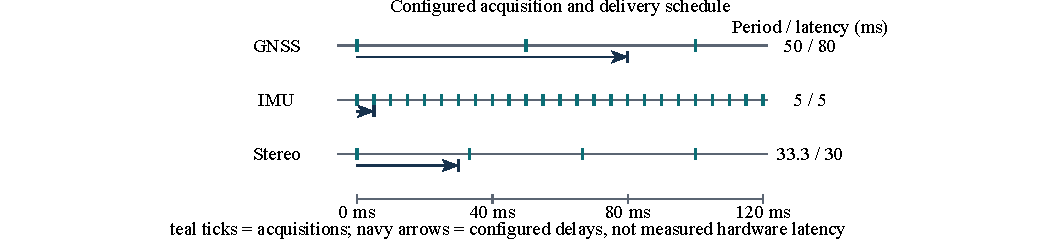
\includegraphics[width=\linewidth]{simulator_report/figures/standalone/05_sensor_timing.pdf}
\caption{Acquisition ticks and configured delivery delays for the three independent sensor streams.}
\label{fig:sens-timing}
\end{figure}


\subsection{GNSS position, velocity, and heading}

GNSS samples the vessel reference pose and body velocity, then rotates those quantities into the east-north frame. The configurable antenna location lies a distance \(\ell\) forward or aft along the boat axis. Let \((x,y,\psi)\) denote vessel reference position and heading, \((u,v)\) body surge and sway speed, and \(r\) yaw rate. The antenna position and velocity are

\begin{equation}
x_{a} = x + \ell\cos\psi,\quad y_{a} = y + \ell\sin\psi,
\end{equation} \begin{equation}
v_{a,e} = u\cos\psi - v\sin\psi - \ell r\sin\psi,\quad v_{a,n} = u\sin\psi + v\cos\psi + \ell r\cos\psi.
\end{equation}

\begin{itemize}
\item
  \texttt{antenna\_lever\_arm} selects \(\ell = \text{gnss\_x\_m}\); otherwise \(\ell = 0\).

  \begin{itemize}
  \item
    The default configured offset is \(- 0.5\) m, so the antenna is behind the reference point. Rotation contributes the tangential velocity terms proportional to \(\ell r\).
  \item
    GNSS heading is the simulated \(\psi\) with configured heading noise. The selected Mosaic-H is a dual-antenna heading receiver; a geometric baseline measurement can be represented as \(\psi = \operatorname{atan2}\left( \Delta_{N},\Delta_{E} \right)\), where \(\left( \Delta_{E},\Delta_{N} \right)\) is the baseline vector between antennas. Baseline heading is not separately simulated.
  \end{itemize}
\item
  Position, velocity, and heading are one named measurement record.

  \begin{itemize}
  \item
    Default standard deviations are 0.02 m per position coordinate, 0.03 m/s per earth-frame velocity coordinate, and 0.15 degrees for heading. The configuration calls its solution mode \texttt{RTK\_FIXED}; it does not model solution-mode transitions.
  \item
    Default position bias is zero. Configurable east and north biases and an optional antenna lever arm affect generated values when their flags are enabled.
  \end{itemize}
\end{itemize}

\subsection{Planar inertial measurements}

The inertial channel reports yaw rate and body-frame specific acceleration at the vessel reference point. Its acceleration equations preserve the rotating body-frame kinematics, so directly exposing derivatives of \(u\) and \(v\) would omit the centripetal coupling terms.

\begin{equation}
\omega_{z} = r,\quad f_{x} = \dot{u} - vr,\quad f_{y} = \dot{v} + ur.
\end{equation}

\begin{itemize}
\item
  The channel samples at 200 Hz by default and reports \(\omega_{z}\), \(f_{x}\), and \(f_{y}\).

  \begin{itemize}
  \item
    Configured white-noise standard deviations are 0.002 rad/s for yaw rate and 0.02 m/s\textsuperscript{2} for each acceleration component.
  \item
    Yaw-rate bias defaults to 0.001 rad/s. Acceleration bias is zero in this model.
  \end{itemize}
\item
  The accelerometer values are computed from the planar physics derivative at acquisition time.

  \begin{itemize}
  \item
    Gravity projection, roll and pitch, sensor-axis misalignment, scale factors, and temperature effects are not represented.
  \item
    This output is suitable as an estimator input, but the simulator supplies no attitude filter or inertial integration.
  \end{itemize}
\end{itemize}

\subsection{Stereo target range and bearing}

The camera abstraction uses a configured static world target and pinhole stereo geometry. It computes ideal target image center and disparity from truth, applies configured pixel noise, and converts those measurements to range and bearing. It does not produce image frames or perform detection, matching, or perception \cite{Stereolabs2026ZEDX}.

The default target is at east-north coordinates \((15,3)\) m, while the initial vessel pose is \((0,0,0)\), so the initial target lies 15 m forward and 3 m to port. The resulting 15.3 m horizontal range is within the configured 20 m validity limit and projects inside the 1920 px image.

For world target \(\left( X_{T},Y_{T} \right)\) and boat pose \((x,y,\psi)\), define forward depth \(Z\) and lateral offset \(Y\) in the boat frame. The true horizontal range and bearing are \(R = \sqrt{Z^{2} + Y^{2}}\) and \(\beta = \operatorname{atan2}(Y,Z)\). The image center coordinate \(c\) and stereo disparity \(d\) follow

\begin{equation}
c = c_{0} - f_{x}\frac{Y}{Z},\quad d = f_{x}\frac{B}{Z},
\end{equation}

where \(c_{0}\) is half the image width, \(f_{x}\) is focal length in pixels, and \(B\) is stereo baseline. The noisy pixel coordinate produces \(\hat{\beta} = \operatorname{atan}\left( \frac{c_{0} - \hat{c}}{f_{x}} \right)\). The model recovers horizontal range as \(\hat{R} = f_{x}\frac{B}{\left\lbrack \hat{d}\cos(\hat{\beta}) \right\rbrack}\).

\begin{itemize}
\item
  A sample is geometrically valid only when depth and disparity are positive, the noisy target center lies within the configured image width, the target range is no greater than 20 m, and the configured occlusion window is inactive.

  \begin{itemize}
  \item
    Random dropout can invalidate an otherwise valid observation. Invalid measurements retain their keys but carry missing values.
  \item
    Default focal length is 700 px, baseline is 0.12 m, image width is 1920 px, center-coordinate noise is 2 px, and disparity noise is 0.5 px.
  \end{itemize}
\item
  Disparity uncertainty produces rapidly growing range uncertainty.

  \begin{itemize}
  \item
    For a front-facing target with small bearing error, \(R \approx Z = f_{x}\frac{B}{d}\). Linearizing this inverse-depth relation gives \(\sigma_{R} \approx Z^{2}\frac{\sigma_{d}}{f_{x}B}\).
  \item
    The plotted curve uses configured \(f_{x}\), \(B\), and \(\sigma_{d}\) and spans the valid 20 m range for an on-axis target. It defines uncertainty as one standard deviation from disparity noise alone; pixel-center noise contributes additional bearing and horizontal-range error off the centerline.
  \end{itemize}
\end{itemize}


\begin{figure}[H]
\centering
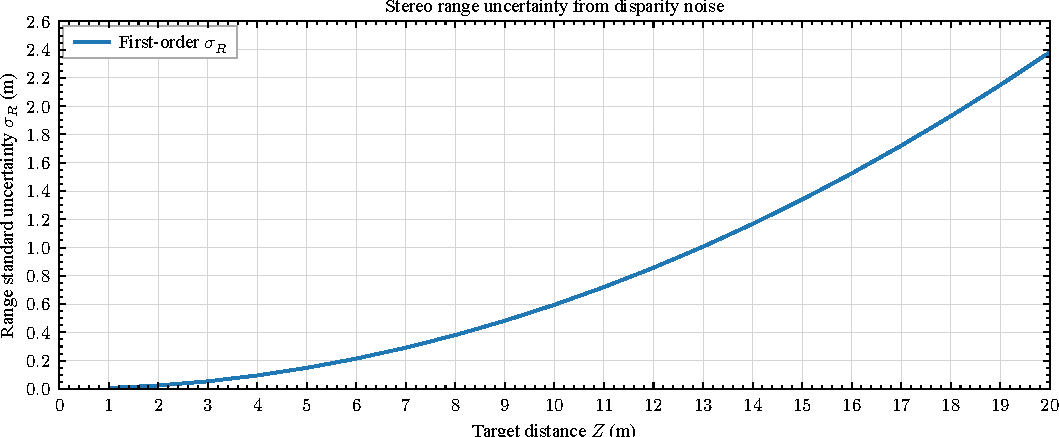
\includegraphics[width=\linewidth]{simulator_report/figures/standalone/06_stereo_uncertainty.pdf}
\caption{First-order stereo range standard uncertainty from the configured disparity noise and camera geometry.}
\label{fig:sens-range-error}
\end{figure}


At 10 m, the model predicts disparity \(700\frac{0.12}{10} = 8.4\) px and first-order range standard uncertainty of about 0.60 m. At 20 m, disparity falls to 4.2 px while uncertainty grows to about 2.38 m. These values expose a geometry limit for downstream estimation; they are not output from image processing or a camera noise experiment.

\subsection{Timing, uncertainty, and estimation boundary}

The defaults below combine rates, delay settings, and noise scales from \texttt{Sensors}. Latency affects when a sample becomes visible, while uncertainty affects its value at acquisition. Each feature is gated independently by the corresponding experiment flags.


{\footnotesize
\setlength{\tabcolsep}{5pt}
\renewcommand{\arraystretch}{1.18}
\begin{longtable}{@{}>{\raggedright\arraybackslash}p{\dimexpr0.23810\linewidth-2\tabcolsep\relax}>{\raggedright\arraybackslash}p{\dimexpr0.17857\linewidth-2\tabcolsep\relax}>{\raggedright\arraybackslash}p{\dimexpr0.21429\linewidth-2\tabcolsep\relax}>{\raggedright\arraybackslash}p{\dimexpr0.36905\linewidth-2\tabcolsep\relax}@{}}
\toprule
Stream & Rate & Latency & Default value uncertainty \\
\midrule
\endfirsthead
\toprule
Stream & Rate & Latency & Default value uncertainty \\
\midrule
\endhead
\bottomrule
\endfoot
GNSS & 20 Hz & 80 ms & 0.02 m; 0.03 m/s; 0.15 deg \\
\addlinespace[3pt]
Inertial & 200 Hz & 5 ms & 0.002 rad/s; 0.02 m/s\textsuperscript{2} \\
\addlinespace[3pt]
Stereo & 30 Hz & 30 ms & 0.5 px disparity; 2 px center \\
\end{longtable}
}


\begin{reportnote}

Rates and latencies are configuration values. The standard deviations are injected only when sensor\_noise is enabled; biases, delay, and random dropout likewise require their respective flags.

\end{reportnote}

An acquisition record stores sample time, availability time, validity, delivered values, and the separate truth used to generate those values. The scheduler exposes only the latest delivered measurement per stream to a policy, so stale and delayed observations are distinguishable from the current state. Independent random streams let noise and dropout draws remain reproducible without coupling one sensor's samples to another's.

\begin{itemize}
\item
  Measurement history supports direct comparison against truth for scoring and debugging.

  \begin{itemize}
  \item
    Invalid samples are recorded and delivered with missing values, preserving the timing of a lost update.
  \item
    A pending sample is not available before its scheduled delivery time, even though its acquisition truth is already logged for evaluation.
  \end{itemize}
\item
  State estimation remains a consumer responsibility.

  \begin{itemize}
  \item
    GNSS provides intermittent pose and earth-frame velocity, while the inertial stream supplies fast body motion cues and stereo supplies target-relative geometry.
  \item
    A filter would need to handle asynchronous sample times, lever-arm corrections, noise and bias, and delayed or missing updates. The simulator does not combine these records into a fused state estimate.
  \end{itemize}
\end{itemize}

\section{Configuration and reproducible operation}\label{cfg-chapter}

The preceding chapters define the implemented physics and observations. Configuration selects which of those mechanisms participates in a run and supplies its numerical parameters. Flags choose a mechanism; parameters determine its strength, timing, and geometry.

\subsection{Configuration hierarchy}

\begin{itemize}
\item
  \texttt{Experiment} supplies the run name, duration, seed, operating point, initial state, and command scenario.

  \begin{itemize}
  \item
    The default run lasts 12 s, starts at 1 m/s, and uses a 5 ms maximum integration step with 20 ms logging.

    \begin{itemize}
    \item
      Sensor and command events split integration intervals at their actual times. The maximum step does not quantize a 35 ms command delay into an approximate event.
    \end{itemize}
  \end{itemize}
\item
  Five nested groups describe the model.

  \begin{itemize}
  \item
    \texttt{flags} contains 31 Boolean switches. \texttt{hull}, \texttt{actuator}, \texttt{environment}, and \texttt{sensors} contain numerical settings.

    \begin{itemize}
    \item
      Disabled effects retain their parameter values so a paired experiment can enable them without silently changing another assumption.
    \end{itemize}
  \end{itemize}
\item
  Full JSON templates define every preset.

  \begin{itemize}
  \item
    \texttt{00\_linear} through \texttt{07\_uncertainty} contain resolved settings rather than hidden inheritance.

    \begin{itemize}
    \item
      The configuration saved with a result is the final version after command-line overrides. Use that record to reproduce a run.
    \end{itemize}
  \end{itemize}
\end{itemize}

\begin{reportnote}

A true flag can produce no numerical effect when its magnitude is zero. For example, enabled sensor dropout with probability zero retains all samples. Always inspect the resolved flag and its associated magnitude together.

\end{reportnote}

\subsection{Preset ladder}

The presets collect related effects into a cumulative ladder. Each row adds the named mechanisms to the preceding configuration. Custom JSON files can select other valid combinations, and isolated comparison mode adds one group to the linear baseline with its required dependencies.


{\footnotesize
\setlength{\tabcolsep}{5pt}
\renewcommand{\arraystretch}{1.18}
\begin{longtable}{@{}>{\raggedright\arraybackslash}p{\dimexpr0.19122\linewidth-2\tabcolsep\relax}>{\raggedright\arraybackslash}p{\dimexpr0.80878\linewidth-2\tabcolsep\relax}@{}}
\toprule
Preset & Additional effects \\
\midrule
\endfirsthead
\toprule
Preset & Additional effects \\
\midrule
\endhead
\bottomrule
\endfoot
\texttt{00\_linear} & Local hull and actuator linearizations; ideal command execution and enabled sensors. Perfect-state access is available. \\
\addlinespace[3pt]
\texttt{01\_hull} & Actual heading rotation, nonlinear velocity coupling, and quadratic hull drag. \\
\addlinespace[3pt]
\texttt{02\_m200} & Signed installed M200 lookup, saturation, neutral deadband, and reverse asymmetry. \\
\addlinespace[3pt]
\texttt{03\_motor} & Motor force lag and force slew limits. \\
\addlinespace[3pt]
\texttt{04\_timing} & Command sampling and compute, transport, and actuation delay. \\
\addlinespace[3pt]
\texttt{05\_sensors} & Measurement noise, bias, latency, GNSS lever arm, and camera occlusion. Perfect-state access is disabled. \\
\addlinespace[3pt]
\texttt{06\_disturbances} & Wind, correlated gusts, apparent wind, wind moment, and prescribed planar wave forcing. \\
\addlinespace[3pt]
\texttt{07\_uncertainty} & Added inertia, motor mismatch, timing jitter, missed commands, watchdog, and random sensor loss. \\
\end{longtable}
}


\begin{itemize}
\item
  A cumulative comparison reveals the response of an increasingly detailed model.

  \begin{itemize}
  \item
    Its last row contains every preceding effect, so the final trajectory difference is not a single-feature result.

    \begin{itemize}
    \item
      An isolated comparison is the appropriate first check when asking which mechanism caused a change.
    \end{itemize}
  \end{itemize}
\item
  Independent flags enable more focused studies than the preset ladder.

  \begin{itemize}
  \item
    For example, retain the nonlinear M200 lookup while disabling only motor lag, or increase GNSS noise while retaining fixed latency.

    \begin{itemize}
    \item
      The numerical values and command tape must remain matched to interpret the resulting difference.
    \end{itemize}
  \end{itemize}
\end{itemize}

\subsection{Complete Boolean flag reference}

The tables below specify the enabled behavior. Baseline means \texttt{00\_linear}; only the three sensor-enable flags and perfect-state feedback are true in that baseline.


{\footnotesize
\setlength{\tabcolsep}{5pt}
\renewcommand{\arraystretch}{1.18}
\begin{longtable}{@{}>{\raggedright\arraybackslash}p{\dimexpr0.27620\linewidth-2\tabcolsep\relax}>{\raggedright\arraybackslash}p{\dimexpr0.72380\linewidth-2\tabcolsep\relax}@{}}
\toprule
Hull switch & Enabled behavior \\
\midrule
\endfirsthead
\toprule
Hull switch & Enabled behavior \\
\midrule
\endhead
\bottomrule
\endfoot
\texttt{nonlinear\_kinematics} & Use the actual heading rotation instead of its local first-order approximation. \\
\addlinespace[3pt]
\texttt{nonlinear\_coupling} & Retain velocity-product coupling instead of its tangent at the operating speed. \\
\addlinespace[3pt]
\texttt{nonlinear\_drag} & Retain quadratic surge drag and any configured quadratic sway/yaw damping. \\
\addlinespace[3pt]
\texttt{added\_mass} & Add separately scaled surge, sway, and yaw inertia and their consistent coupling. \\
\end{longtable}
}



{\footnotesize
\setlength{\tabcolsep}{5pt}
\renewcommand{\arraystretch}{1.18}
\begin{longtable}{@{}>{\raggedright\arraybackslash}p{\dimexpr0.27620\linewidth-2\tabcolsep\relax}>{\raggedright\arraybackslash}p{\dimexpr0.72380\linewidth-2\tabcolsep\relax}@{}}
\toprule
Propulsion switch & Enabled behavior \\
\midrule
\endfirsthead
\toprule
Propulsion switch & Enabled behavior \\
\midrule
\endhead
\bottomrule
\endfoot
\texttt{nonlinear\_thrust} & Use the bounded, signed installed-scaled M200 lookup. Requires saturation. \\
\addlinespace[3pt]
\texttt{thrust\_saturation} & Clip force to the selected forward/reverse bounds. Input percentages always stay within -100\% through +100\%. \\
\addlinespace[3pt]
\texttt{neutral\_deadband} & Set requested force to zero for commands from -6.25\% through +6.25\%. \\
\addlinespace[3pt]
\texttt{reverse\_asymmetry} & Use the weaker reverse branch. With a linear actuator, scale negative force by the reverse/forward limit ratio. \\
\addlinespace[3pt]
\texttt{motor\_lag} & Apply first-order force response using the configured time constant. \\
\addlinespace[3pt]
\texttt{motor\_rate\_limit} & Limit force change per second; combine with lag when both are enabled. \\
\addlinespace[3pt]
\texttt{motor\_mismatch} & Apply separate motor gains and retain force limits when saturation is enabled. \\
\end{longtable}
}



{\footnotesize
\setlength{\tabcolsep}{5pt}
\renewcommand{\arraystretch}{1.18}
\begin{longtable}{@{}>{\raggedright\arraybackslash}p{\dimexpr0.27620\linewidth-2\tabcolsep\relax}>{\raggedright\arraybackslash}p{\dimexpr0.72380\linewidth-2\tabcolsep\relax}@{}}
\toprule
Timing switch & Enabled behavior \\
\midrule
\endfirsthead
\toprule
Timing switch & Enabled behavior \\
\midrule
\endhead
\bottomrule
\endfoot
\texttt{command\_sampling} & Read the input program or call a policy on periodic command ticks. \\
\addlinespace[3pt]
\texttt{command\_delay} & Queue computation, transport, and actuation dead time before applying the command. \\
\addlinespace[3pt]
\texttt{timing\_jitter} & Add bounded nonnegative delay. Requires command sampling and delay. \\
\addlinespace[3pt]
\texttt{missed\_commands} & Drop individual command updates with the selected probability. Requires sampling. \\
\addlinespace[3pt]
\texttt{command\_watchdog} & Request neutral after no command has been applied for the timeout. Requires sampling. \\
\end{longtable}
}



{\footnotesize
\setlength{\tabcolsep}{5pt}
\renewcommand{\arraystretch}{1.18}
\begin{longtable}{@{}>{\raggedright\arraybackslash}p{\dimexpr0.27620\linewidth-2\tabcolsep\relax}>{\raggedright\arraybackslash}p{\dimexpr0.72380\linewidth-2\tabcolsep\relax}@{}}
\toprule
Environmental switch & Enabled behavior \\
\midrule
\endfirsthead
\toprule
Environmental switch & Enabled behavior \\
\midrule
\endhead
\bottomrule
\endfoot
\texttt{wind} & Apply projected-area aerodynamic force from the configured world-frame wind. \\
\addlinespace[3pt]
\texttt{gusts} & Add a seeded correlated wind-velocity process. Requires wind. \\
\addlinespace[3pt]
\texttt{apparent\_wind} & Subtract boat translational velocity before evaluating aerodynamic loading. Requires wind. \\
\addlinespace[3pt]
\texttt{wind\_yaw\_moment} & Apply wind force at an offset to obtain yaw moment. Requires wind. \\
\addlinespace[3pt]
\texttt{wave\_forcing} & Add prescribed sinusoidal planar force/moment. Independent of wind. \\
\end{longtable}
}



{\footnotesize
\setlength{\tabcolsep}{5pt}
\renewcommand{\arraystretch}{1.18}
\begin{longtable}{@{}>{\raggedright\arraybackslash}p{\dimexpr0.27620\linewidth-2\tabcolsep\relax}>{\raggedright\arraybackslash}p{\dimexpr0.72380\linewidth-2\tabcolsep\relax}@{}}
\toprule
Sensor / observation switch & Enabled behavior \\
\midrule
\endfirsthead
\toprule
Sensor / observation switch & Enabled behavior \\
\midrule
\endhead
\bottomrule
\endfoot
\texttt{sensor\_noise} & Add separate GNSS, inertial, pixel-center, and disparity noise streams. \\
\addlinespace[3pt]
\texttt{sensor\_bias} & Add configured GNSS position offsets and gyro bias. \\
\addlinespace[3pt]
\texttt{sensor\_delay} & Queue measurements until their sensor availability times. \\
\addlinespace[3pt]
\texttt{sensor\_dropout} & Invalidate randomly selected samples using separate probabilities per sensor. \\
\addlinespace[3pt]
\texttt{antenna\_lever\_arm} & Include the GNSS antenna offset in its position and velocity. \\
\addlinespace[3pt]
\texttt{camera\_occlusion} & Invalidate target observations during the configured time interval. \\
\addlinespace[3pt]
\texttt{gnss\_enabled} & Schedule GNSS acquisition and delivery. True in the baseline. \\
\addlinespace[3pt]
\texttt{imu\_enabled} & Schedule inertial acquisition and delivery. True in the baseline. \\
\addlinespace[3pt]
\texttt{camera\_enabled} & Schedule camera acquisition and delivery. True in the baseline. \\
\addlinespace[3pt]
\texttt{perfect\_state\_feedback} & Expose a separate exact state tuple to a policy. True in the baseline; false from the sensor preset onward. \\
\end{longtable}
}


\subsection{Useful numerical controls}

With the enable switches defined, numerical overrides allow sensitivity studies without editing the implementation. The values below are default test settings; they are not a component acceptance specification.


{\footnotesize
\setlength{\tabcolsep}{5pt}
\renewcommand{\arraystretch}{1.18}
\begin{longtable}{@{}>{\raggedright\arraybackslash}p{\dimexpr0.21955\linewidth-2\tabcolsep\relax}>{\raggedright\arraybackslash}p{\dimexpr0.63881\linewidth-2\tabcolsep\relax}>{\raggedright\arraybackslash}p{\dimexpr0.14164\linewidth-2\tabcolsep\relax}@{}}
\toprule
Group & Principal controls & Default \\
\midrule
\endfirsthead
\toprule
Group & Principal controls & Default \\
\midrule
\endhead
\bottomrule
\endfoot
Run & Duration / integration step / log interval. & 12 s / 5 ms / 20 ms. \\
\addlinespace[3pt]
Operating point & Forward speed / heading. & 1 m/s / 0 rad. \\
\addlinespace[3pt]
Hull & Mass, inertia, and each drag scale. & 1.0 each. \\
\addlinespace[3pt]
Added inertia & Surge / sway / yaw fractions. & 0.10 / 0.50 / 0.20. \\
\addlinespace[3pt]
Geometry & Motor separation / GNSS forward offset. & 0.75 m / -0.50 m. \\
\addlinespace[3pt]
Motor & Force time constant / force slew limit. & 0.20 s / 80 N/s. \\
\addlinespace[3pt]
Command & Period / compute / transport / dead time. & 20 / 5 / 10 / 20 ms. \\
\addlinespace[3pt]
Command failure & Maximum jitter / watchdog timeout. & 3 ms / 100 ms. \\
\addlinespace[3pt]
Wind & Speed / direction / gust standard deviation. & 5 m/s / 90\textdegree{} / 0.5 m/s. \\
\addlinespace[3pt]
Gust & Correlation time / process sample period. & 1 s / 0.1 s. \\
\addlinespace[3pt]
Wave forcing & Surge / sway / yaw amplitude, period. & 0 N / 1 N / 0.1 N m, 4 s. \\
\end{longtable}
}


\begin{itemize}
\item
  Hull controls include separate linear and quadratic surge scales, linear sway and yaw scales, optional quadratic sway/yaw damping, and added-inertia fractions.

  \begin{itemize}
  \item
    Changing an inertia fraction does not change hull mass or nominal drag.

    \begin{itemize}
    \item
      Changing mass scale also changes the geometric yaw-inertia proxy. Change inertia scale independently to study mass-distribution error.
    \end{itemize}
  \end{itemize}
\item
  Actuator controls include individual motor gains, all timing intervals, and missed-command probability.

  \begin{itemize}
  \item
    The uncertainty preset uses gains 0.95 and 1.05 and missed-command probability 0.02.

    \begin{itemize}
    \item
      Other presets retain gains and probabilities but leave their corresponding effects disabled.
    \end{itemize}
  \end{itemize}
\item
  Sensor controls include periods, latency, each noise magnitude, bias, dropout probability, geometry, and occlusion interval.

  \begin{itemize}
  \item
    The uncertainty preset uses GNSS dropout probability 0.05 and camera dropout probability 0.10. Inertial dropout remains zero.

    \begin{itemize}
    \item
      A camera target is a fixed world point with configurable east/north position. It is not a generated competition scene.
    \end{itemize}
  \end{itemize}
\end{itemize}

\subsection{Reproduce a run and change one assumption}

Run the commands from \texttt{EMCH792/projects/boat\_control}. The first example repeats the report demonstration; the second makes a controlled sensor change.

\begin{minipage}{\linewidth}
\begin{verbatim}
uv sync
uv run python -m blueboat_sim compare \
  --set command_amplitude_percent=20 \
  --output build/configurable-simulator

uv run python -m blueboat_sim run --preset 05_sensors \
  --set sensors.gnss_position_sigma_m=0.10 \
  --set flags.sensor_dropout=true \
  --set sensors.gnss_dropout_probability=0.05 \
  --set seed=100 --output build/noisy-run
\end{verbatim}
\end{minipage}

\begin{itemize}
\item
  Use \texttt{-\/-set\ group.field=value} for a numerical or Boolean override.

  \begin{itemize}
  \item
    Boolean values use JSON \texttt{true} or \texttt{false}; a textual string is rejected as a flag.

    \begin{itemize}
    \item
      Unknown keys, invalid probabilities, nonfinite values, reversed occlusion intervals, and inconsistent flag dependencies are rejected before integration.
    \end{itemize}
  \end{itemize}
\item
  Use a custom JSON file when several related settings change together.

  \begin{itemize}
  \item
    \texttt{-\/-config\ configs/simulator/05\_sensors.json} supplies a complete template.

    \begin{itemize}
    \item
      Repeated \texttt{-\/-config} arguments compare custom templates in their supplied order. Duration, scenario, operating point, command amplitude, and initial state must match.
    \end{itemize}
  \end{itemize}
\item
  Use a command tape when the input must be exactly specified.

  \begin{itemize}
  \item
    \texttt{configs/simulator/commands/reversal.json} requests neutral, full forward, full reverse, and neutral at 0, 2, 4, and 6 s.

    \begin{itemize}
    \item
      Commands start at zero, use finite port/starboard percentages within -100\% to +100\%, and have strictly increasing times within the run.
    \end{itemize}
  \end{itemize}
\end{itemize}

\subsection{Outputs, auditing, and numerical limits}

The command tape defines the requested excitation. Logs then expose the sequence between that request and the observed motion, so a run can be inspected rather than judged only by its final plot.


{\footnotesize
\setlength{\tabcolsep}{5pt}
\renewcommand{\arraystretch}{1.18}
\begin{longtable}{@{}>{\raggedright\arraybackslash}p{\dimexpr0.21955\linewidth-2\tabcolsep\relax}>{\raggedright\arraybackslash}p{\dimexpr0.78045\linewidth-2\tabcolsep\relax}@{}}
\toprule
Saved file & Use \\
\midrule
\endfirsthead
\toprule
Saved file & Use \\
\midrule
\endhead
\bottomrule
\endfoot
\texttt{resolved\_config.json} & Reproduce all final settings after overrides. \\
\addlinespace[3pt]
\texttt{input\_tape.json} & Inspect the common requested motor-percentage changes. \\
\addlinespace[3pt]
\texttt{truth.csv} & Plot time, six hull states, two actual motor forces, applied percentages, device pulse widths, and target force. \\
\addlinespace[3pt]
\texttt{metrics.json} & Compare scalar summaries under the declared experiment. \\
\addlinespace[3pt]
\texttt{result.json} & Audit physical parameters, source hash, trim, raw sensor records, command application, watchdog trips, and policy decision timestamps. \\
\addlinespace[3pt]
\texttt{comparison.json} & Store matched histories and GNSS records for downstream plots; each record marks whether it was delivered. \\
\addlinespace[3pt]
\texttt{summary.json} & Locate run directories and their metrics. \\
\end{longtable}
}


\begin{itemize}
\item
  Each output directory is named from the run name and seed.

  \begin{itemize}
  \item
    Reusing the same directory replaces that run's files.

    \begin{itemize}
    \item
      Use a new output root to retain an earlier experiment. Seeds support repeatability within the numerical environment; archive software versions for long-term reproduction.
    \end{itemize}
  \end{itemize}
\item
  Hull states use fourth-order Runge-Kutta integration between exact event boundaries.

  \begin{itemize}
  \item
    Motor force uses the analytic held-target lag/ramp solution at each stage.

    \begin{itemize}
    \item
      Event times and integration step serve different purposes. Reduce the maximum step for numerical convergence while retaining the physical sensor and command periods.
    \end{itemize}
  \end{itemize}
\item
  The validator caps a run at two million nominal integration steps and two million estimated scheduled events.

  \begin{itemize}
  \item
    Nonfinite integrated states raise an error.

    \begin{itemize}
    \item
      A successful run is still inspected for bounds, equilibrium behavior, and step-size convergence. Completion alone does not establish accuracy.
    \end{itemize}
  \end{itemize}
\end{itemize}

\section{Experiments, Disturbances, and Validation}

\subsection{Experiment design and comparisons}

The comparison runner applies a common command record to configurations that share duration, scenario, operating point, amplitude, and initial state. The saved experiment lasts \(12\) s, uses a \(5\) ms integration step, and begins at \((x,y,\psi,u,v,r) = (0,0,0,1,0,0)\) in SI units. Each configuration receives the same four-event pulse-and-turn input tape, and seed \(792\) is used throughout.

\begin{itemize}
\item
  The tape starts at trim, raises both motor commands by \(20\) percentage points at \(t = 2\) s, creates a differential command at \(t = 4\) s, and returns to trim at \(t = 6\) s.

  \begin{itemize}
  \item
    Reusing the tape makes each run a controlled open-loop comparison under identical requested inputs.
  \item
    Comparing internal motor force as well as position separates command interpretation and actuator response from hull and environmental effects.
  \end{itemize}
\item
  The cumulative mode enables successive groups of model features on top of each preceding stage.

  \begin{itemize}
  \item
    The saved order is linear baseline, nonlinear hull, installed motor map, motor response, timing, sensors, disturbances, and parameter uncertainty.
  \item
    A late-stage displacement therefore reflects the accumulated configuration; it cannot be attributed to that stage alone.
  \end{itemize}
\item
  Paired seeds preserve each named random stream across the compared configurations, while separate streams isolate gust, sensor, and timing draws.

  \begin{itemize}
  \item
    This reduces avoidable randomness in the comparison, but a single seed does not characterize run-to-run variability.
  \item
    Isolated mode adds each feature group to the same baseline, which is preferable when estimating that group's marginal effect.
  \end{itemize}
\end{itemize}


\begin{figure}[H]
\centering
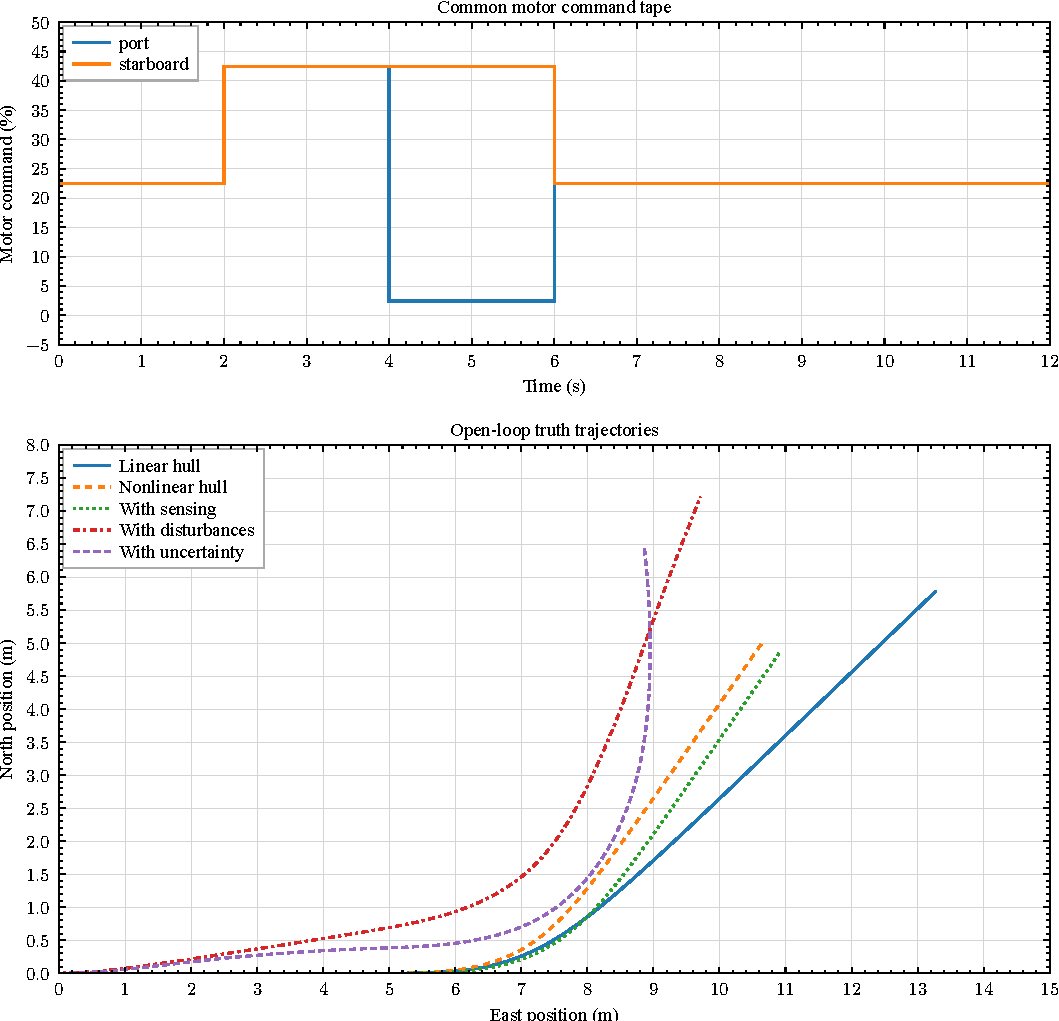
\includegraphics[width=\linewidth]{simulator_report/figures/standalone/07_command_tape_paths.pdf}
\caption{The common input tape and selected truth trajectories show how cumulative model stages change open-loop response.}
\label{fig:exp-input-path}
\end{figure}


The trajectory legend maps Linear hull to \texttt{00\_linear}, Nonlinear hull to \texttt{01\_hull}, With sensing to \texttt{05\_sensors}, With disturbances to \texttt{06\_disturbances}, and With uncertainty to \texttt{07\_uncertainty}.

\subsection{Wind and prescribed waves}

Environmental forcing enters the planar equations as body-frame surge force \(X\), sway force \(Y\), and yaw moment \(N\). The configured steady wind vector is expressed in earth axes and can include two correlated gust components. With apparent wind enabled, the vessel's earth-frame velocity is subtracted before the relative wind is rotated into body axes.

For heading \(\psi\), earth-frame wind \(\left( w_{E},w_{N} \right)\), and body velocities \((u,v)\), the relative wind is \(w_{r}^{e} = \left( w_{E},w_{N} \right) - R(\psi)(u,v)\), where \(R(\psi)\) rotates body components into earth axes. The model then rotates \(w_{r}^{e}\) back into body axes as \(\left( w_{x},w_{y} \right)\). Its axis-wise projected-area drag is

\begin{equation}
\left( X_{w},Y_{w} \right) = \frac{1}{2}\rho_{a}C_{D}\left( A_{f}w_{x}|w_{x}|,A_{l}w_{y}|w_{y}| \right),
\end{equation}

where \(\rho_{a}\) is air density, \(C_{D}\) is the configured coefficient, and \(A_{f},A_{l}\) are frontal and lateral projected areas. If the force is applied at configured body offset \(\left( x_{c},y_{c} \right)\), its yaw moment is \(N_{w} = x_{c}Y_{w} - y_{c}X_{w}\). The saved setting places the wind center \(0.1\) m forward and on the centerline, so lateral wind force produces a yaw moment while surge force does not.

\begin{itemize}
\item
  Gusts follow a first-order update for two independently driven, temporally correlated components at the configured \(0.1\) s interval.

  \begin{itemize}
  \item
    For interval \(\Delta t\) and correlation time \(\tau_{g}\), \(g_{\left\{ k + 1 \right\}} = ag_{k} + \sigma_{g}\sqrt{1 - a^{2}}\eta_{k}\), with \(a = \exp( - \Delta\frac{t}{\tau_{g}})\) and independent unit-normal two-axis draw \(\eta_{k}\).
  \item
    Linear interpolation between update times makes the applied wind continuous in time; it does not make the gust process a measured atmospheric record.
  \end{itemize}
\item
  The wave option adds sinusoidal components \(\left\lbrack X_{q},Y_{q},N_{q} \right\rbrack = \left\lbrack A_{X},A_{Y},A_{N} \right\rbrack\sin(2\pi\frac{t}{T_{q}})\) directly to the three generalized forces.

  \begin{itemize}
  \item
    In the saved disturbance stage, the wave amplitudes are \(0\) N surge, \(1\) N sway, and \(0.1\) N m yaw with a \(4\) s period.
  \item
    This prescribed planar forcing omits wave propagation, encounter frequency, heave, roll, pitch, and hydrodynamic radiation or diffraction, so it is a repeatable disturbance input rather than a sea-state simulation.
  \end{itemize}
\end{itemize}

The feature set therefore supports repeatable sensitivity experiments. Its wind drag is an engineering approximation and its wave term is prescribed; neither establishes disturbance fidelity for a particular field condition.

\subsection{Reading the saved run}

The input tape produces clear cumulative changes in the east-north truth paths. The baseline travels \(13.28\) m east and \(5.79\) m north by \(12\) s. The nonlinear-hull stage ends at \((10.65,5.01)\) m, showing that the same motor-percentage tape can produce a different path when the dynamics change. The sensor stage overlays the timing-stage truth, while prescribed disturbances move the endpoint to \((9.71,7.21)\) m and uncertainty moves it to \((8.86,6.46)\) m. Those endpoints describe the supplied experiment and are not evidence of improved tracking or a better controller.


\begin{figure}[H]
\centering
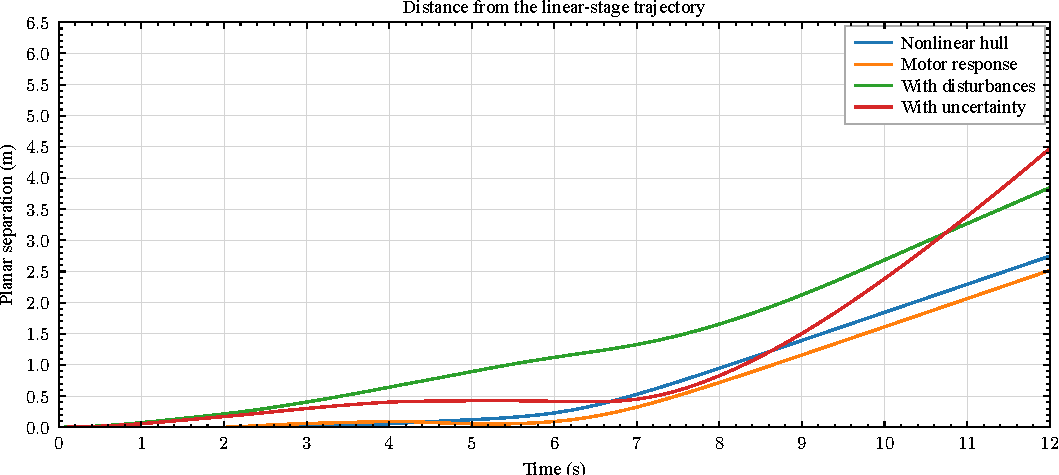
\includegraphics[width=\linewidth]{simulator_report/figures/standalone/08_stage_offsets.pdf}
\caption{Selected cumulative-stage separation from the linear baseline under the same open-loop trial.}
\label{fig:exp-stage-offset}
\end{figure}


The following values are read from the saved comparison record; the force integral is the time integral of the sum of squared port and starboard thrust, not mechanical work or energy.


{\footnotesize
\setlength{\tabcolsep}{5pt}
\renewcommand{\arraystretch}{1.18}
\begin{longtable}{@{}>{\raggedright\arraybackslash}p{\dimexpr0.26549\linewidth-2\tabcolsep\relax}>{\raggedright\arraybackslash}p{\dimexpr0.14159\linewidth-2\tabcolsep\relax}>{\raggedright\arraybackslash}p{\dimexpr0.14159\linewidth-2\tabcolsep\relax}>{\raggedright\arraybackslash}p{\dimexpr0.13274\linewidth-2\tabcolsep\relax}>{\raggedright\arraybackslash}p{\dimexpr0.15929\linewidth-2\tabcolsep\relax}>{\raggedright\arraybackslash}p{\dimexpr0.15929\linewidth-2\tabcolsep\relax}@{}}
\toprule
Stage & Final E (m) & Final N (m) & Peak (N) & \(\int\lVert T\rVert^2\,dt\) (N\textsuperscript{2} s) & GNSS RMS (m) \\
\midrule
\endfirsthead
\toprule
Stage & Final E (m) & Final N (m) & Peak (N) & \(\int\lVert T\rVert^2\,dt\) (N\textsuperscript{2} s) & GNSS RMS (m) \\
\midrule
\endhead
\bottomrule
\endfoot
00 linear & 13.28 & 5.79 & 14.69 & 2080 & 0.000 \\
\addlinespace[3pt]
01 hull & 10.65 & 5.01 & 14.69 & 2080 & 0.000 \\
\addlinespace[3pt]
02 motor map & 10.82 & 5.08 & 15.46 & 2219 & 0.000 \\
\addlinespace[3pt]
03 motor response & 10.92 & 4.92 & 15.46 & 2168 & 0.000 \\
\addlinespace[3pt]
04 timing & 10.94 & 4.89 & 15.46 & 2168 & 0.000 \\
\addlinespace[3pt]
05 sensors & 10.94 & 4.89 & 15.46 & 2168 & 0.029 \\
\addlinespace[3pt]
06 disturbances & 9.71 & 7.21 & 15.46 & 2168 & 0.029 \\
\addlinespace[3pt]
07 uncertainty & 8.86 & 6.46 & 16.24 & 2224 & 0.029 \\
\end{longtable}
}


\protect\phantomsection\label{exp-metrics}{}

In this table, \(T\) is the two-element vector of motor thrusts, and \(\int\lVert T\rVert^2\,dt\) has units N\textsuperscript{2} s. It is a command-effort proxy useful for comparing force histories; calling it energy would require multiplying force by velocity in a physically consistent power calculation. The sensor stage introduces a GNSS position RMS error of \(0.029\) m while leaving truth nearly coincident with the timing-stage path. Sensor noise, bias, delay, dropout, and acquisition latency alter delivered observations and their scoring against truth; they do not feed back into the open-loop state integration when the applied command tape is fixed.

\subsection{Validation scope and next experiments}

The existing tests check implementation behavior. They verify deterministic random streams, force and motor calculations, command timing, sensor causality, feature isolation, and the invariant that sensor errors do not change open-loop truth. These checks establish software properties for the implemented equations and scheduling logic. They do not measure agreement with a physical boat.

\begin{itemize}
\item
  The reported GNSS position error compares the delivered measurement's position with the truth at that measurement's acquisition time.

  \begin{itemize}
  \item
    The truth point is the GNSS antenna location, including the configured lever arm, rather than the vessel reference origin.
  \item
    Delivery latency determines when a controller could receive the record; it does not change the acquisition timestamp used for measurement error.
  \end{itemize}
\item
  A field-oriented identification study should collect synchronized PWM, GNSS, inertial, and motor or current records under documented loading and environmental conditions.

  \begin{itemize}
  \item
    Estimate surge, sway, yaw, motor-map, lag, and rate parameters from selected maneuvers, then freeze those values before evaluation.
  \item
    Hold out complete sessions, routes, and environmental conditions so adjacent samples from one maneuver do not leak across fit and test partitions.
  \end{itemize}
\item
  Future closed-loop controller comparisons should report tracking error, cross-track error, heading error, settling and overshoot, actuator saturation, force effort, and robustness across held-out seeds and conditions.

  \begin{itemize}
  \item
    Score navigation against acquisition-time truth and separately report observation age and dropout so estimation error and communications delay remain distinguishable.
  \item
    These are proposed validation measures; the saved runs do not compare controllers or demonstrate performance gains.
  \end{itemize}
\end{itemize}

\begin{reportnote}

The current evidence supports reproducible software tests and controlled model comparisons. Physical parameter identification and held-out boat trials are required to establish predictive accuracy.

\end{reportnote}

\clearpage

\section{Complete parameter reference}\label{param-chapter}

The flag catalog selects behavior, while this reference records every non-Boolean field in the baseline JSON template. Values are generated directly from that template to keep the report aligned with its runnable configuration. Field names preserve the command-line spelling. Numerical values are rounded to six decimal places here; the saved JSON retains their full precision.

\begin{itemize}
\item
  The baseline keeps most physical effects disabled while retaining their numerical settings.

  \begin{itemize}
  \item
    Enabling a flag activates its associated values without replacing them.

    \begin{itemize}
    \item
      The cumulative uncertainty preset changes three probabilities. Missed commands become 0.02, GNSS dropout becomes 0.05, and camera dropout becomes 0.10. It also disables perfect-state feedback as inherited from the sensor stage.
    \end{itemize}
  \end{itemize}
\item
  Each group below supplies the prefix used in \texttt{-\/-set\ group.field=value}.

  \begin{itemize}
  \item
    Top-level experiment settings use \texttt{-\/-set\ field=value}.

    \begin{itemize}
    \item
      The initial-state sequence is ordered \(x,y,\psi,u,v,r\). A custom initial velocity does not automatically change the operating-point trim used to initialize motor force.
    \end{itemize}
  \end{itemize}
\item
  Camera geometry and measurement-error fields specify this simulator abstraction.

  \begin{itemize}
  \item
    They do not replace camera calibration, noise characterization, or receiver status logs.

    \begin{itemize}
    \item
      Delay, noise, bias, dropout, and disturbance magnitudes become physical claims only after identification under documented conditions.
    \end{itemize}
  \end{itemize}
\end{itemize}

\subsection{Experiment settings}


{\footnotesize
\setlength{\tabcolsep}{5pt}
\renewcommand{\arraystretch}{1.18}
\begin{longtable}{@{}>{\raggedright\arraybackslash}p{\dimexpr0.38952\linewidth-2\tabcolsep\relax}>{\raggedright\arraybackslash}p{\dimexpr0.15581\linewidth-2\tabcolsep\relax}>{\raggedright\arraybackslash}p{\dimexpr0.45467\linewidth-2\tabcolsep\relax}@{}}
\toprule
Field & Default value & Unit / kind \\
\midrule
\endfirsthead
\toprule
Field & Default value & Unit / kind \\
\midrule
\endhead
\bottomrule
\endfoot
\texttt{name} & 00\_linear & dimensionless / identifier \\
\addlinespace[3pt]
\texttt{duration\_s} & 12.0 & s \\
\addlinespace[3pt]
\texttt{integration\_step\_s} & 0.005 & s \\
\addlinespace[3pt]
\texttt{log\_period\_s} & 0.02 & s \\
\addlinespace[3pt]
\texttt{seed} & 792 & dimensionless / identifier \\
\addlinespace[3pt]
\texttt{operating\_speed\_m\_s} & 1.0 & m/s \\
\addlinespace[3pt]
\texttt{operating\_heading\_rad} & 0.0 & rad \\
\addlinespace[3pt]
\texttt{initial\_state} & 0.0, 0.0, 0.0, 1.0, 0.0, 0.0 & m, m, rad, m/s, m/s, rad/s \\
\addlinespace[3pt]
\texttt{scenario} & turn & dimensionless / identifier \\
\addlinespace[3pt]
\texttt{command\_amplitude\_percent} & 2.5 & percentage points \\
\end{longtable}
}


\subsection{Hull parameters}


{\footnotesize
\setlength{\tabcolsep}{5pt}
\renewcommand{\arraystretch}{1.18}
\begin{longtable}{@{}>{\raggedright\arraybackslash}p{\dimexpr0.38952\linewidth-2\tabcolsep\relax}>{\raggedright\arraybackslash}p{\dimexpr0.15581\linewidth-2\tabcolsep\relax}>{\raggedright\arraybackslash}p{\dimexpr0.45467\linewidth-2\tabcolsep\relax}@{}}
\toprule
Field & Default value & Unit / kind \\
\midrule
\endfirsthead
\toprule
Field & Default value & Unit / kind \\
\midrule
\endhead
\bottomrule
\endfoot
\texttt{mass\_scale} & 1.0 & dimensionless / identifier \\
\addlinespace[3pt]
\texttt{inertia\_scale} & 1.0 & dimensionless / identifier \\
\addlinespace[3pt]
\texttt{thruster\_spacing\_m} & 0.75 & m \\
\addlinespace[3pt]
\texttt{surge\_linear\_scale} & 1.0 & dimensionless / identifier \\
\addlinespace[3pt]
\texttt{surge\_quadratic\_scale} & 1.0 & dimensionless / identifier \\
\addlinespace[3pt]
\texttt{sway\_linear\_scale} & 1.0 & dimensionless / identifier \\
\addlinespace[3pt]
\texttt{yaw\_linear\_scale} & 1.0 & dimensionless / identifier \\
\addlinespace[3pt]
\texttt{sway\_quadratic\_N\_s2\_m2} & 0.0 & N s\textsuperscript{2}/m\textsuperscript{2} \\
\addlinespace[3pt]
\texttt{yaw\_quadratic\_N\_m\_s2} & 0.0 & N m s\textsuperscript{2} \\
\addlinespace[3pt]
\texttt{added\_surge\_fraction} & 0.1 & dimensionless / identifier \\
\addlinespace[3pt]
\texttt{added\_sway\_fraction} & 0.5 & dimensionless / identifier \\
\addlinespace[3pt]
\texttt{added\_yaw\_fraction} & 0.2 & dimensionless / identifier \\
\end{longtable}
}


\subsection{Actuator and command parameters}


{\footnotesize
\setlength{\tabcolsep}{5pt}
\renewcommand{\arraystretch}{1.18}
\begin{longtable}{@{}>{\raggedright\arraybackslash}p{\dimexpr0.38952\linewidth-2\tabcolsep\relax}>{\raggedright\arraybackslash}p{\dimexpr0.15581\linewidth-2\tabcolsep\relax}>{\raggedright\arraybackslash}p{\dimexpr0.45467\linewidth-2\tabcolsep\relax}@{}}
\toprule
Field & Default value & Unit / kind \\
\midrule
\endfirsthead
\toprule
Field & Default value & Unit / kind \\
\midrule
\endhead
\bottomrule
\endfoot
\texttt{lag\_s} & 0.2 & s \\
\addlinespace[3pt]
\texttt{rate\_limit\_N\_s} & 80.0 & N/s \\
\addlinespace[3pt]
\texttt{port\_gain} & 0.95 & dimensionless / identifier \\
\addlinespace[3pt]
\texttt{starboard\_gain} & 1.05 & dimensionless / identifier \\
\addlinespace[3pt]
\texttt{command\_period\_s} & 0.02 & s \\
\addlinespace[3pt]
\texttt{compute\_delay\_s} & 0.005 & s \\
\addlinespace[3pt]
\texttt{transport\_delay\_s} & 0.01 & s \\
\addlinespace[3pt]
\texttt{dead\_time\_s} & 0.02 & s \\
\addlinespace[3pt]
\texttt{jitter\_max\_s} & 0.003 & s \\
\addlinespace[3pt]
\texttt{missed\_command\_probability} & 0.0 & dimensionless / identifier \\
\addlinespace[3pt]
\texttt{command\_timeout\_s} & 0.1 & s \\
\end{longtable}
}


\subsection{Environmental parameters}


{\footnotesize
\setlength{\tabcolsep}{5pt}
\renewcommand{\arraystretch}{1.18}
\begin{longtable}{@{}>{\raggedright\arraybackslash}p{\dimexpr0.38952\linewidth-2\tabcolsep\relax}>{\raggedright\arraybackslash}p{\dimexpr0.15581\linewidth-2\tabcolsep\relax}>{\raggedright\arraybackslash}p{\dimexpr0.45467\linewidth-2\tabcolsep\relax}@{}}
\toprule
Field & Default value & Unit / kind \\
\midrule
\endfirsthead
\toprule
Field & Default value & Unit / kind \\
\midrule
\endhead
\bottomrule
\endfoot
\texttt{wind\_speed\_m\_s} & 5.0 & m/s \\
\addlinespace[3pt]
\texttt{wind\_direction\_deg} & 90.0 & deg \\
\addlinespace[3pt]
\texttt{wind\_drag\_coefficient} & 1.0 & dimensionless / identifier \\
\addlinespace[3pt]
\texttt{frontal\_area\_m2} & 0.18 & m\textsuperscript{2} \\
\addlinespace[3pt]
\texttt{lateral\_area\_m2} & 0.3 & m\textsuperscript{2} \\
\addlinespace[3pt]
\texttt{wind\_center\_x\_m} & 0.1 & m \\
\addlinespace[3pt]
\texttt{wind\_center\_y\_m} & 0.0 & m \\
\addlinespace[3pt]
\texttt{gust\_sigma\_m\_s} & 0.5 & m/s \\
\addlinespace[3pt]
\texttt{gust\_correlation\_s} & 1.0 & s \\
\addlinespace[3pt]
\texttt{gust\_period\_s} & 0.1 & s \\
\addlinespace[3pt]
\texttt{wave\_surge\_N} & 0.0 & N \\
\addlinespace[3pt]
\texttt{wave\_sway\_N} & 1.0 & N \\
\addlinespace[3pt]
\texttt{wave\_yaw\_N\_m} & 0.1 & N m \\
\addlinespace[3pt]
\texttt{wave\_period\_s} & 4.0 & s \\
\end{longtable}
}


\clearpage
\subsection{Sensor parameters}


{\footnotesize
\setlength{\tabcolsep}{5pt}
\renewcommand{\arraystretch}{1.18}
\begin{longtable}{@{}>{\raggedright\arraybackslash}p{\dimexpr0.38952\linewidth-2\tabcolsep\relax}>{\raggedright\arraybackslash}p{\dimexpr0.15581\linewidth-2\tabcolsep\relax}>{\raggedright\arraybackslash}p{\dimexpr0.45467\linewidth-2\tabcolsep\relax}@{}}
\toprule
Field & Default value & Unit / kind \\
\midrule
\endfirsthead
\toprule
Field & Default value & Unit / kind \\
\midrule
\endhead
\bottomrule
\endfoot
\texttt{gnss\_period\_s} & 0.05 & s \\
\addlinespace[3pt]
\texttt{imu\_period\_s} & 0.005 & s \\
\addlinespace[3pt]
\texttt{camera\_period\_s} & 0.033333 & s \\
\addlinespace[3pt]
\texttt{gnss\_delay\_s} & 0.08 & s \\
\addlinespace[3pt]
\texttt{imu\_delay\_s} & 0.005 & s \\
\addlinespace[3pt]
\texttt{camera\_delay\_s} & 0.03 & s \\
\addlinespace[3pt]
\texttt{gnss\_position\_sigma\_m} & 0.02 & m \\
\addlinespace[3pt]
\texttt{gnss\_velocity\_sigma\_m\_s} & 0.03 & m/s \\
\addlinespace[3pt]
\texttt{gnss\_heading\_sigma\_rad} & 0.002618 & rad \\
\addlinespace[3pt]
\texttt{gyro\_sigma\_rad\_s} & 0.002 & rad/s \\
\addlinespace[3pt]
\texttt{acceleration\_sigma\_m\_s2} & 0.02 & m/s\textsuperscript{2} \\
\addlinespace[3pt]
\texttt{gyro\_bias\_rad\_s} & 0.001 & rad/s \\
\addlinespace[3pt]
\texttt{gnss\_bias\_e\_m} & 0.0 & m \\
\addlinespace[3pt]
\texttt{gnss\_bias\_n\_m} & 0.0 & m \\
\addlinespace[3pt]
\texttt{gnss\_dropout\_probability} & 0.0 & dimensionless / identifier \\
\addlinespace[3pt]
\texttt{imu\_dropout\_probability} & 0.0 & dimensionless / identifier \\
\addlinespace[3pt]
\texttt{camera\_dropout\_probability} & 0.0 & dimensionless / identifier \\
\addlinespace[3pt]
\texttt{gnss\_x\_m} & -0.5 & m \\
\addlinespace[3pt]
\texttt{camera\_fx\_px} & 700.0 & px \\
\addlinespace[3pt]
\texttt{camera\_width\_px} & 1920.0 & px \\
\addlinespace[3pt]
\texttt{camera\_baseline\_m} & 0.12 & m \\
\addlinespace[3pt]
\texttt{camera\_disparity\_sigma\_px} & 0.5 & px \\
\addlinespace[3pt]
\texttt{camera\_center\_sigma\_px} & 2.0 & px \\
\addlinespace[3pt]
\texttt{camera\_max\_range\_m} & 20.0 & m \\
\addlinespace[3pt]
\texttt{occlusion\_start\_s} & 5.0 & s \\
\addlinespace[3pt]
\texttt{occlusion\_end\_s} & 6.0 & s \\
\addlinespace[3pt]
\texttt{target\_e\_m} & 15.0 & m \\
\addlinespace[3pt]
\texttt{target\_n\_m} & 3.0 & m \\
\end{longtable}
}


\clearpage
\bibliographystyle{unsrtnat}
\bibliography{references}
\end{document}
